\chapter{A Taxonomy of Collective Decision Procedures}
\label {apx:taxonomy-of-collective-decision-procedures}

Collective decision procedures, as described by Nicolaus Tideman \autocite[9-21]{Tideman2006}, are divided into two families, as shown in \prettyref{fig:ao-collective-decision-taxonomy}: agreement-on-outcome and agreement-on-procedure.



\begin{figure}[t]
    \centering
    \begin{tikzpicture}[
        %sibling distance=10em,
        font=\small,
        edge from parent path={(\tikzchildnode.north) -- ++(0,0.5cm)
            -| (\tikzparentnode.south)},
        level distance=1.75cm,
        every node/.style = {
            shape=rectangle, rounded corners,
            draw=blue!75,
            align=center,
            top color=white,
            bottom color=blue!20,
            drop shadow}
        ]

        \draw (0,0) [sibling distance=15em] node {Collective Decision Procedures}
            child { [sibling distance=5em, level distance=3.5cm] node (AOO) {Agreement on Outcome}
                child[grow=down,xshift=-2.5cm] { [level distance=1.75cm] node {Consensus}
                    child { node {Discovered\\Consensus} }
                    child { node {Achieved\\Consensus} }
                }
                child[grow=down,xshift=1.9cm] { [level distance=1.75cm] node {Pseudo-consensus}
                    child { node {Immediate\\Pseudo-\\consensus} }
                    child { node {Achieved\\Pseudo-\\consensus} }
                }
                child[grow=down,xshift=6.15cm] { [level distance=1.75cm] node {Trade}
                    child { node {Purchase} }
                    child { node {Negotiated\\Exchange} }
                }
                child[grow=down,xshift=10.5cm] { [level distance=1.75cm] node {Extortion}
                    child { node {Hold-up} }
                    child { node {Treaty} }
                }
            }
            child { [sibling distance=5em] node {Agreement on Procedure}
                [edge from parent fork down]
                child { node {Authority} }
                child { node {Random\\Process} }
                child { node {Voting} }
                child { node {Contest} }
            };
%        \Tree
%            [.{Collective Decision Procedures}
%                [.{Agreement on Outcome}
%                    [.{Consensus}
%                        [.{Discovered\\Consensus} ]
%                        [.{Achieved\\Consensus} ]
%                    ]
%                    [.{Pseudo-consensus}
%                        [.{Immediate\\Pseudo-consensus} ]
%                        [.{Achieved\\Pseudo-consensus} ]
%                    ]
%                ]
%                [.{Agreement on Procedure}
%                    [.Authority ]
%                    [.{Random\\Process} ]
%                    [.Voting ]
%                    [.Contest ]
%                ]
%            ]

    \end{tikzpicture}
    \caption{\label{fig:ao-collective-decision-taxonomy}A taxonomy of collective decision procedures \autocite[14]{Tideman2006}.}
\end{figure}

\begin{definition}{Agreement on Procedure}
    A collective decision procedure for which the collectivity has agreed to abide by the outcome.
\end{definition}

Agreement on procedure is recognizable in Democratic governments, which grant \textit{authority} to legislatures, executives, and judges through elections (\textit{voting}) and appointments.  Legislators make laws by \textit{voting}, while judges have authority in deciding criminal cases, torts, and even the legitimacy of laws under the rules set forth by a Constitution.

Popular sovereignty means the \textit{authority} for these Constitutional rules comes from the consent of the governed.  Those governed by Constitutions must consent to these Constitutional rules, generally achieved by a process of \textit{voting} on the initial adoption and further amendments.  This raises a question:  what does \textit{consent} mean?


\begin{figure}[t]
    \centering
    \begin{tikzpicture}
        % Put Compensation (Absent) at origin plus a little movement back.
        % Square
        \draw (3cm,1cm) node (Compensation) {Compensation}
        (Compensation) ++(-3,0) node (CompensationAbsent) {}
        ++(0,0.5) node {Absent}
        (Compensation) ++(3,0) node (CompensationPresent) {}
        ++(0,0.5) node {Present};


        \draw (-2.5,0) ++(0,-2.5cm) node (Dissatisfaction) {Dissatisfaction}
        (Dissatisfaction) ++(0,2.5cm) node (DissatisfactionAbsent) {Absent}
        (Dissatisfaction) ++(0,-2.5) node (DissatisfactionPresent) {Present};

        \foreach \x in {Compensation,Dissatisfaction}
        \foreach \y in {Absent,Present}
        {
            \draw [->,>=latex] (\x) -- (\x\y);
        }

        \node (Box) at (0,0) {};

        \draw (Box) node [align=center] (Consensus) {Consensus}
        ++(6cm,0) node [align=center] (Trade) {Trade}
        ++(0,-5cm) node[align=center] (Extortion) {Extortion}
        ++(-6cm,0) node[align=center] (PConsensus) {Pseudo-\\consensus};

        \foreach \x[remember=\x as \lastx (initially PConsensus)] in {Consensus,Trade,Extortion,PConsensus}
        {
            \draw (\lastx) -- (\x);
        }
    \end{tikzpicture}
    \caption{\label{fig:ao-outcome-modes}Locations of modes in the agreement-on-outcome family \autocite[14]{Tideman2006}.}
\end{figure}

\prettyref{fig:ao-outcome-modes} shows the modes of agreement on outcome.  All of these require unanimous consent:  every party must accept the rules or else they have no power.  The rules may include a procedure for further decisions, which binds the collectivity to its agreement.  Once a collectivity has decided on its Constitutional rules, its members have unanimously agreed to abide by them, and so consent to the processes and procedures set forth therein.

\begin{definition}{Agreement on Outcome}
    A collective decision procedure by which every member of the collectivity must agreed to the chosen actions.
\end{definition}

The modes of agreement on outcome are characterized by the presence or lack of compensation and dissatisfaction in a decision by unanimous consent.  For example, a group has \textit{consensus} if all its members agree that the decision is what should be done or what they want to be done, while \textit{pseudo-consensus} occurs when some members agree to the action despite not agreeing with the decision \textit{and are not compensated}.  By contrast, individuals are compensated under \textit{extortion}, but disagree with the actions of others in the group during the decision process.

\begin{commentary}{Extortion in Ancient Rome}
    Extortion occurs when someone threatens you or otherwise coerces you into action.  While you might quickly agree to their demands, their behavior is generally considered wrong and often illegal.

    Contracts under duress are frequently considered invalid.  This was not the case in ancient Rome during the time Crassus operated his fire brigade, which would negotiate \textit{during} the fire for services in exchange for ownership of the house.
\end{commentary}

\textit{Consensus} and \textit{trade} both imply satisfaction, while \textit{trade} and \textit{extortion} both imply compensation.  The difference is that trade is voluntary, and more specifically that no party feels any other party has acted inappropriately.

Tidemean expands these four modes further as shown in \prettyref{fig:ao-outcome-submodes}, based on the amount of effort, essentially discussion and negotiation.


\begin{figure}[t]
    \centering
    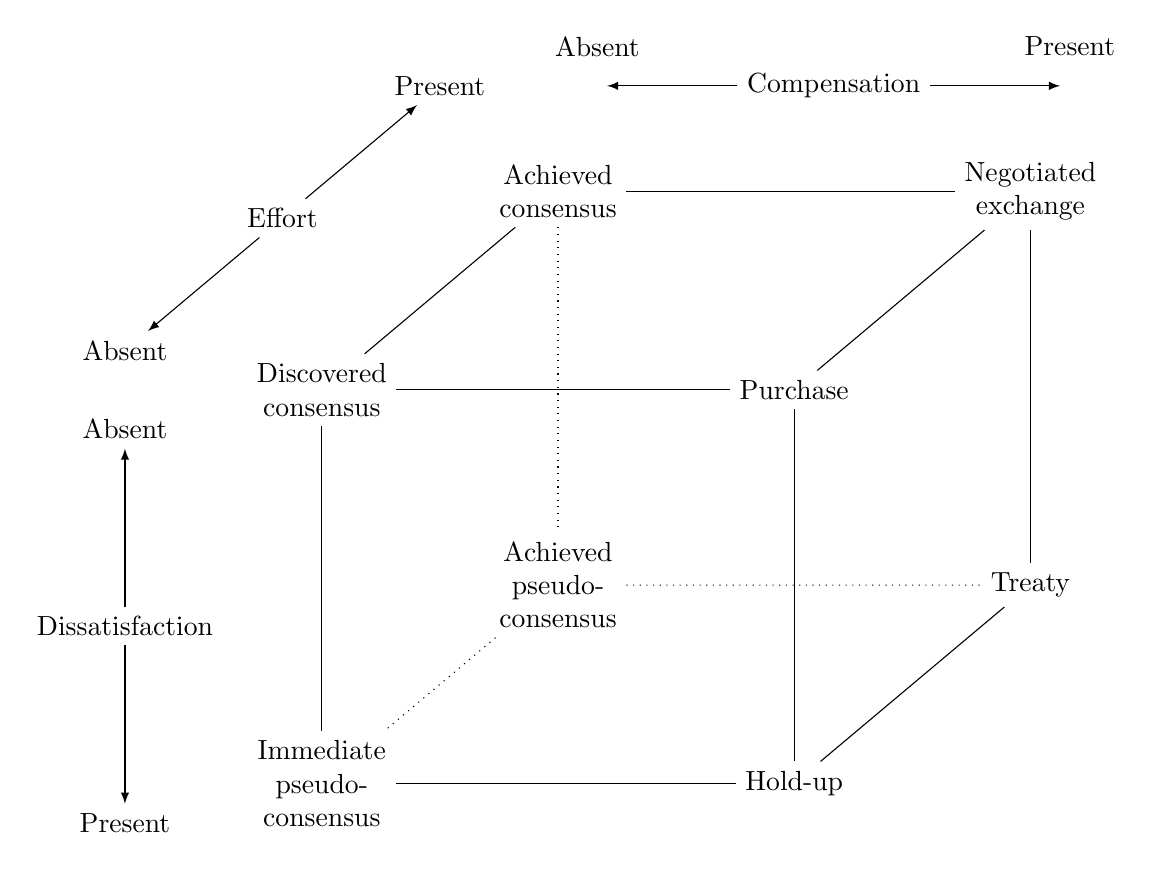
\begin{tikzpicture}
        % Put Effort (Absent) at origin plus a little movement back.
        % Cube corner is at origin
        % 40 degrees e.g. tan(40 degrees) * x = y
        \draw (-2.5,0.5) ++(2cm,1.68cm) node (Effort) {Effort};
        \draw (Effort) ++(-2cm,-1.68cm) node (EffortAbsent) {Absent}
              (Effort) ++(2cm,1.68cm) node (EffortPresent) {Present};

        \draw (EffortPresent) ++(5cm,0) node (Compensation) {Compensation}
              (Compensation) ++(-3,0) node (CompensationAbsent) {}
              ++(0,0.5) node {Absent}
              (Compensation) ++(3,0) node (CompensationPresent) {}
              ++(0,0.5) node {Present};


        \draw (-2.5,-0.5) ++(0,-2.5cm) node (Dissatisfaction) {Dissatisfaction}
            (Dissatisfaction) ++(0,2.5cm) node (DissatisfactionAbsent) {Absent}
            (Dissatisfaction) ++(0,-2.5) node (DissatisfactionPresent) {Present};

        \foreach \x in {Compensation,Effort,Dissatisfaction}
        \foreach \y in {Absent,Present}
        {
            \draw [->,>=latex] (\x) -- (\x\y);
        }

        \node (Cube) at (0,0) {};

        \draw (Cube) node [align=center] (DiscoveredConsensus) {Discovered \\ consensus}
            ++(3cm,2.52cm) node [align=center] (AchievedConsensus) {Achieved \\ consensus}
            ++(6cm,0) node [align=center] (NegotiatedExchange) {Negotiated \\ exchange}
            (DiscoveredConsensus) ++(6cm,0) node[align=center] (Purchase) {Purchase}
            (DiscoveredConsensus) ++(0,-5cm) node[align=center] (ImmediatePC) {Immediate \\ pseudo-\\consensus}
            (Purchase) ++(0,-5cm) node[align=center] (HoldUp) {Hold-up}
            (NegotiatedExchange) ++(0,-5cm) node[align=center] (Treaty) {Treaty}
            (AchievedConsensus) ++(0,-5) node[align=center] (AchievedPC) {Achieved\\pseudo-\\consensus};

        \foreach \x[remember=\x as \lastx (initially Purchase)] in {DiscoveredConsensus,AchievedConsensus,NegotiatedExchange,Purchase,HoldUp,Treaty,NegotiatedExchange}
        {
            \draw (\lastx) -- (\x);
        }
        \foreach \x[remember=\x as \lastx (initially DiscoveredConsensus)] in {ImmediatePC,HoldUp}
        {
            \draw (\lastx) -- (\x);
        }
        \foreach \x[remember=\x as \lastx (initially AchievedConsensus)] in {AchievedPC,Treaty}
        {
            \draw [dotted] (\lastx) -- (\x);
        }
        \foreach \x[remember=\x as \lastx (initially AchievedPC)] in {ImmediatePC}
        {
            \draw [dotted] (\lastx) -- (\x);
        }
    \end{tikzpicture}
    \caption{\label{fig:ao-outcome-submodes}Locations of sub-modes in the agreement-on-outcome family \autocite[15]{Tideman2006}.}
\end{figure}

\begin{definition}{Effort and Coercion}
%    The two sub-modes of trade, purchase and negotiated exchange, show the negotiation aspect of achieving effort.  If you've ever made a large purchase, you've probably done more than just showing up with money.  Sellers will bundle services or products and offer discount packages as a simple purchase, but more major purchases involve sales representatives and repeated calls to management to authorize discounts.  Different clients get different levels of discount not only dependent on the size of the purchase, but on the degree of leverage they bring to the negotiating table.

%    Even though a buyer may have leverage, such as the ability to walk away from the deal and buy a competitor's product, the seller in such purchases cannot be coerced.  By contrast, if the buyer \textit{needs} the product, the seller can use this need to drive the buyer to the highest price they're willing to pay by threatening to walk away themselves—simply by refusing a lower bid.  Such cases are frequently called ``price gouging'' and fall under extortion.

%   A treaty implies coercion, as well.  In a neutral state, trade is free flowing and military conflicts are nonexistent.  A treaty is the negotiation of the conditions under which trade will remain free and military conflicts will be avoided, implying that there will be consequences if an agreement is not reached.  Treaties almost exclusively arise when some or all parties feel the others have acted inappropriately.  Peace treaties are negotiated between parties with ongoing or recent military conflicts and the threat of further military action.

Effort and coercion make the difference between the sub-modes of trade and extortion.  With trade, you can walk into a store and make a purchase; but for large deals, a lot of negotiation can go into obtaining long-term contracts, guaranteed supply chains, and discounts.  Extortion is similar:  under a hold-up, someone issues threats and both parties quickly agree to an action; whereas treaties always come with the threat of military action or economic barriers, and nevertheless involve long negotiations to improve the outcomes for all parties.
\end{definition}

Kassner argues democratic procedures only retain legitimacy by their alignment with normative democratic ideals \autocite{Kassner2006}.  We can extend this to a requirement to actively pursue processes and procedures which maximize the representativeness of the voters, such that if a process is known and can be accepted by the individuals of the collectivity, then it must be implemented if it can be shown and agreed to be the most maximizing such system.  Inherently, this means the voters must be able to understand and verify the process, or verify that it can be verified with special knowledge and without special permission, and that it is the duty of political leaders to work toward voter education to bring voters to understand and accept such systems which can satisfy all of these requirements.

\clearpage
\begin{definition}{Voting}
    A collective decision procedure by which, on the basis of a previous collective decision, a set of possible options is identified for consideration, the members of the collectivity report one or more aspects of their evaluation of these options, and an outcome is selected on the basis of a mathematical function of these reports \autocite{Tideman2006}.
\end{definition}

Tideman defines voting as an agreed-upon procedure such that, if the procedure is not carried out as the collectivity has agreed, the decision has not been made by voting.  There are many forms of ballots and many tabulation methods to determine an outcome from these ballots; these often produce different results based on what information for which they account, and how they account for it.  For example, a plurality vote elects by the largest faction in agreement on the best option; whereas a Condorcet system elects based on pairwise contests—typically expressed by ranked ballots—such that an option must have majority support over each competing option individually.

